\centering
\section*{\myul{Grundlagen}}

\begin{tikzpicture}[remember picture, overlay]

% --- ERSTE REIHE: Am Seitenursprung anfangen
\setlength{\rowheight}{126.4mm}

    % A1) Erste Kachel relativ zum Seitenursprung
    \setlength{\cellwidth}{190mm}
    \Tile{A1}{([xshift=10mm, yshift=-18mm]current page.north west)}{\cellwidth}{\rowheight}
        {
            \vspace{-2mm}
            \titlebf{Koordinatensysteme}\\ \vspace{2mm}
            \begin{minipage}[t]{0.265\cellwidth-\TileSep}
                \centering
                \titlerm{Kartesische Koordinaten}\\ \vspace{-4mm}
                \begin{align*}
                    v_x &= u \\
                    v_y &= v \\
                    v_z &= w
                \end{align*}%
                \\ \vspace{2mm}
                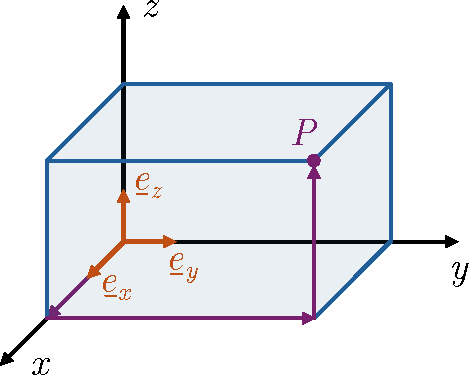
\includegraphics[width=40mm]{images/koordinaten-kartesisch.pdf}\\ \vspace{-2mm}
                \begin{equation*}
                    h_1 = 1 \qquad h_2 = 1 \qquad h_3 = 1
                \end{equation*}
                \vspace{-2mm}
                \begin{equation*}
                    \nabla = \underline{e}_x\,\frac{\partial}{\partial x} + \underline{e}_y\,\frac{\partial}{\partial y} + \underline{e}_z\,\frac{\partial}{\partial z}
                \end{equation*}
                \begin{equation*}
                    \nabla\cdot\underline{v} = \frac{\partial u}{\partial x} + \frac{\partial v}{\partial y} + \frac{\partial w}{\partial z}
                \end{equation*}
                \begin{align*}
                    \left(\nabla\times\underline{v}\right)_x &= \frac{\partial w}{\partial y} - \frac{\partial v}{\partial z} \\
                    \left(\nabla\times\underline{v}\right)_y &= \frac{\partial u}{\partial z} - \frac{\partial w}{\partial x} \\
                    \left(\nabla\times\underline{v}\right)_z &= \frac{\partial v}{\partial x} - \frac{\partial u}{\partial y}
                \end{align*}
                \vspace{-3mm}
            \end{minipage}%
            \vline
            \begin{minipage}[t]{0.29\cellwidth}
                \centering
                \titlerm{Zylinderkoordinaten}\\ \vspace{2mm}
                \begin{minipage}{0.145\cellwidth}
                    \centering
                    \vspace{-3mm}
                    \begin{align*}
                        x &= r\,\cos\!\left(\varphi\right) \\
                        y &= r\,\sin\!\left(\varphi\right) \\
                        z &= z
                    \end{align*}
                \end{minipage}%
                \vline
                \begin{minipage}{0.145\cellwidth}
                    \centering
                    \vspace{-3mm}
                    \begin{align*}
                        r       &= \sqrt{x^2+y^2} \\
                        \varphi &= \arctan\!\left(\tfrac{y}{x}\right) \\
                        z       &= z
                    \end{align*}
                \end{minipage}%
                \\ \vspace{3.5mm}
                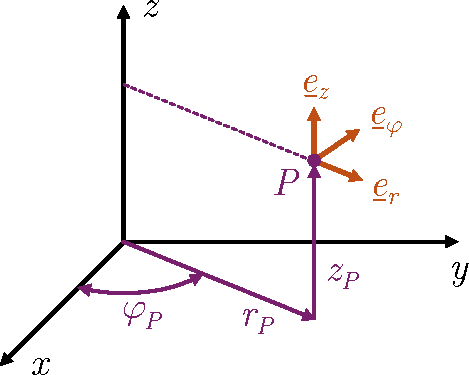
\includegraphics[width=40mm]{images/koordinaten-zylindrisch.pdf}\\ \vspace{-2mm}
                \begin{equation*}
                    h_1 = 1 \qquad h_2 = r \qquad h_3 = 1
                \end{equation*}
                \vspace{-2mm}
                \begin{equation*}
                    \nabla = \underline{e}_r\,\frac{\partial}{\partial r} + \underline{e}_\varphi\,\frac{1}{r}\,\frac{\partial}{\partial \varphi} + \underline{e}_z\,\frac{\partial}{\partial z}
                \end{equation*}
                \begin{equation*}
                    \nabla\cdot\underline{v} = \frac{1}{r}\,\frac{\partial}{\partial r}\left(r\,u\right) + \frac{1}{r}\,\frac{\partial v}{\partial\varphi} + \frac{\partial w}{\partial z}
                \end{equation*}
                \begin{align*}
                    \left(\nabla\times\underline{v}\right)_r       &= \frac{1}{r}\,\frac{\partial w}{\partial\varphi} - \frac{\partial v}{\partial z} \\
                    \left(\nabla\times\underline{v}\right)_\varphi &= \frac{\partial u}{\partial z} - \frac{\partial w}{\partial r} \\
                    \left(\nabla\times\underline{v}\right)_z       &= \frac{1}{r}\,\left[\frac{\partial}{\partial r}\left(r\,u\right) - \frac{\partial u}{\partial\varphi}\right]
                \end{align*}
                \vspace{-3mm}
            \end{minipage}%
            \vline
            \begin{minipage}[t]{0.44\cellwidth-\TileSep}
                \centering
                \titlerm{Kugelkoordinaten}\\ \vspace{1mm}
                \begin{minipage}{0.2\cellwidth}
                    \centering
                    \vspace{-3.5mm}
                    \begin{align*}
                        x &= r\,\sin\!\left(\vartheta\right)\,\cos\!\left(\varphi\right) \\[0.5ex]
                        y &= r\,\sin\!\left(\vartheta\right)\,\sin\!\left(\varphi\right) \\[0.5ex]
                        z &= r\,\cos\!\left(\varphi\right)
                    \end{align*}
                \end{minipage}%
                \vline
                \begin{minipage}{0.2\cellwidth}
                    \centering
                    \vspace{-3mm}
                    \begin{align*}
                        r         &= \sqrt{x^2+y^2+z^2} \\
                        \vartheta &= \arccos\!\left(\tfrac{z}{r}\right) \\
                        \varphi   &= \arccos\!\left(\tfrac{x}{\sqrt{x^2+y^2}}\right)
                    \end{align*}
                \end{minipage}%
                \\ \vspace{1.72mm}
                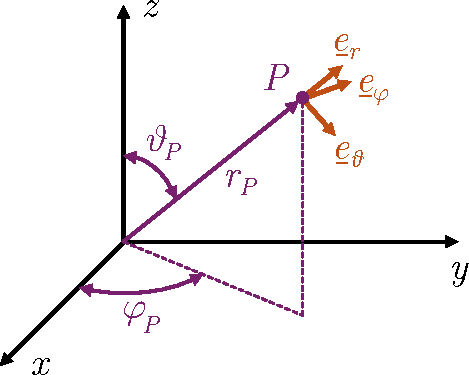
\includegraphics[width=40mm]{images/koordinaten-kugelform.pdf}\\ \vspace{-2mm}
                \begin{equation*}
                    h_1 = 1 \qquad h_2 = r \qquad h_3 = r\,\sin\!\left(\vartheta\right)
                \end{equation*}
                \vspace{-2mm}
                \begin{equation*}
                    \nabla = \underline{e}_r\,\frac{\partial}{\partial r} + \underline{e}_\vartheta\,\frac{1}{r}\,\frac{\partial}{\partial \vartheta} + \underline{e}_\varphi\,\frac{1}{r\,\sin\!\left(\vartheta\right)}\,\frac{\partial}{\partial \varphi}
                \end{equation*}
                \vspace{-0.4mm}
                {\scriptsize
                \begin{equation*}
                    \nabla\cdot\underline{v} = \frac{1}{r^2}\frac{\partial}{\partial r}\!\left(r^2\,u\right) + \frac{1}{r\,\sin\!\left(\vartheta\right)}\frac{\partial}{\partial\varphi}\!\left(v\,\sin\!\left(\vartheta\right)\right) + \frac{1}{r\,\sin\!\left(\vartheta\right)}\frac{\partial w}{\partial\varphi}
                \end{equation*}}
                \vspace{-1.25mm}
                \begin{align*}
                    \left(\nabla\times\underline{v}\right)_r         &= \frac{1}{r\,\sin\!\left(\vartheta\right)}\left[\frac{\partial}{\partial\vartheta}\left(\sin\!\left(\vartheta\right)\,w\right) - \frac{\partial v}{\partial\varphi}\right] \\
                    \left(\nabla\times\underline{v}\right)_\vartheta &= \frac{1}{r\,\sin\!\left(\vartheta\right)}\,\frac{\partial u}{\partial\varphi} - \frac{1}{r}\frac{\partial}{\partial r}\left(r\,w\right) \\[0.5ex]
                    \left(\nabla\times\underline{v}\right)_\varphi   &= \frac{1}{r}\,\left[\frac{\partial}{\partial r}\left(r\,v\right) - \frac{\partial u}{\partial\vartheta}\right]
                \end{align*}
                \vspace{-3mm}
            \end{minipage}
        }{0}{0}{1}{0}

% --- ZWEITE REIHE: Unten anbauen
\setlength{\rowheight}{20mm}

    % A2) Erste Kachel unten anbauen
    \setlength{\cellwidth}{44mm}
    \Tile{A2}{(A1.south west)}{\cellwidth}{\rowheight}
        {
            \titlerm{Skalarprodukt}\vspace{1mm}
            \begin{equation*}
                \underline{a}\cdot\underline{b}
            \end{equation*}
        }{0}{1}{1}{0}

    % B2) Zweite Kachel rechts anbauen
    \setlength{\cellwidth}{42mm}
    \Tile{B2}{(A2.north east)}{\cellwidth}{\rowheight}
        {
            \titlerm{Kreuzprodukt}\vspace{1mm}
            \begin{equation*}
                \underline{a}\times\underline{b}
            \end{equation*}
        }{0}{1}{1}{0}

    % C2) Dritte Kachel rechts anbauen
    \setlength{\cellwidth}{54mm}
    \Tile{C2}{(B2.north east)}{\cellwidth}{\rowheight}
        {
            \titlerm{Dyadisches Produkt}\vspace{1mm}
            \begin{equation*}
                \underline{a}\,\underline{b} = \underline{a}\otimes\underline{b} = \underline{a}\,\underline{b}^\text{T}
            \end{equation*}
        }{0}{1}{1}{0}

    % D2) Vierte Kachel rechts anbauen
    \setlength{\cellwidth}{50mm}
    \Tile{D2}{(C2.north east)}{\cellwidth}{\rowheight}
        {
            \titlerm{Nabla-Operator}\vspace{-2mm}
            \begin{equation*}
                \nabla = \sum_{i=1}^3 \underline{e}_i\,\frac{1}{h_i}\,\frac{\partial}{\partial x_i}
            \end{equation*}
        }{0}{0}{1}{0}

% --- DRITTE REIHE: Unten anbauen
\setlength{\rowheight}{24mm}

    % A3) Erste Kachel unten anbauen
    \setlength{\cellwidth}{110mm}
    \Tile{A3}{(A2.south west)}{\cellwidth}{\rowheight}
        {
            \titlerm{Gradient eines Skalars}\vspace{2mm}
            \begin{equation*}
                \text{grad}\!\left(f\right) = \nabla\!\left(f\right) = \underline{e}_1\,\frac{1}{h_1}\,\frac{\partial f}{\partial x_1} + \underline{e}_2\,\frac{1}{h_2}\,\frac{\partial f}{\partial x_2} + \underline{e}_3\,\frac{1}{h_3}\,\frac{\partial f}{\partial x_3}
            \end{equation*}
        }{0}{1}{1}{0}

    % B3) Zweite Kachel rechts anbauen
    \setlength{\cellwidth}{80mm}
    \Tile{B3}{(A3.north east)}{\cellwidth}{\rowheight}
        {
            \titlerm{Gradient eines Vektors}\vspace{-1.5mm}
            \begin{equation*}
                \text{grad}\!\left(\underline{v}\right) = \nabla\otimes\underline{v} = \left(
                \begin{matrix}
                    \tfrac{\partial u}{\partial x} & \tfrac{\partial v}{\partial x} & \tfrac{\partial w}{\partial x} \\[1.0ex]
                    \tfrac{\partial u}{\partial y} & \tfrac{\partial v}{\partial y} & \tfrac{\partial w}{\partial y} \\[1.0ex]
                    \tfrac{\partial u}{\partial z} & \tfrac{\partial v}{\partial z} & \tfrac{\partial w}{\partial z}
                \end{matrix}\right)
            \end{equation*}
        }{0}{0}{1}{0}

% --- VIERTE REIHE: Unten anbauen
\setlength{\rowheight}{22mm}

    % A4) Erste Kachel unten anbauen
    \setlength{\cellwidth}{190mm}
    \Tile{A4}{(A3.south west)}{\cellwidth}{\rowheight}
        {
            \titlerm{Divergenz}\vspace{1mm}
            \begin{equation*}
                \text{div}\!\left(\underline{a}\right) = \nabla\cdot\underline{a} = \frac{1}{h_1\,h_2\,h_3}\,\left[\frac{\partial}{\partial x_1}\left(h_2\,h_3\,a_1\right) + \frac{\partial}{\partial x_2}\left(h_3\,h_1\,a_2\right) + \frac{\partial}{\partial x_3}\left(h_1\,h_2\,a_3\right)\right]
            \end{equation*}
        }{0}{0}{1}{0}

% --- FÜNFTE REIHE: Unten anbauen
\setlength{\rowheight}{24mm}

    % A5) Erste Kachel unten anbauen
    \setlength{\cellwidth}{190mm}
    \Tile{A5}{(A4.south west)}{\cellwidth}{\rowheight}
        {
            \titlerm{Rotation}\vspace{2mm}
            \begin{equation*}
                \text{rot}\!\left(\underline{a}\right) = \nabla\times\underline{a} = \frac{1}{h_1\,h_2\,h_3}\,\left[h_1\left(\frac{\partial\left(h_3\,a_3\right)}{\partial x_2} - \frac{\partial\left(h_2\,a_2\right)}{\partial x_3}\right)\,\underline{e}_1 + h_2\left(\frac{\partial\left(h_1\,a_1\right)}{\partial x_3} - \frac{\partial\left(h_3\,a_3\right)}{\partial x_1}\right)\,\underline{e}_2 + h_3\left(\frac{\partial\left(h_2\,a_2\right)}{\partial x_1} - \frac{\partial\left(h_1\,a_1\right)}{\partial x_2}\right)\,\underline{e}_3\right]
            \end{equation*}
        }{0}{0}{1}{0}

% --- SECHSTE REIHE: Unten anbauen
\setlength{\rowheight}{24mm}

    % A6) Erste Kachel unten anbauen
    \setlength{\cellwidth}{190mm}
    \Tile{A6}{(A5.south west)}{\cellwidth}{\rowheight}
        {
            \titlerm{Laplace-Operator}\vspace{2mm}
            \begin{equation*}
                \nabla^2\!\left(f\right) = \Delta\!\left(f\right) = \frac{1}{h_1\,h_2\,h_3}\,\left[\frac{\partial}{\partial x_1}\left(\frac{h_2\,h_3}{h_1}\,\frac{\partial f}{\partial x_1}\right) + \frac{\partial}{\partial x_2}\left(\frac{h_3\,h_1}{h_2}\,\frac{\partial f}{\partial x_2}\right) + \frac{\partial}{\partial x_3}\left(\frac{h_1\,h_2}{h_3}\,\frac{\partial f}{\partial x_3}\right)\right]
            \end{equation*}
        }{0}{0}{0}{0}

\end{tikzpicture}